\chapter{Astroparticle Physics} \label{sec:astro}

Cosmic particles have always offered an insight into the mechanisms of cosmic objects.
\todo{Do you need to define what cosmic particles are, or can we assume the reader knows that we mean particles form outside the solar system?}
For example, pulsars and quasars have been discovered through radio astronomy.
\todo{Radio astronomy feels like the most wave-like astronomy we do.}
Today, information is obtained from all kinds of cosmic particles, including weakly interacting neutrinos.
The production of high-energy neutrinos is due to charged particles that have been accelerated by a type of shock front acceleration in magnetic fields.
\todo{What about (suspected) SMBH neutrino emissions?}
These are mainly charged hadronic particles such as protons, which, in the framework of the standard model of particle physics, produces a pion mainly through interaction with other protons (hadronuclear),
\begin{align}
  p+p \rightarrow p+n+\pi^+,
\end{align}
or photons (photohadronic),
\begin{align}
  p\gamma \rightarrow n+\pi^+.
\end{align}
In the course of the pion's decay, neutrinos are ultimately created \cite{pdg},
\begin{align}
  &\pi^+ \rightarrow \mu^++\nu_\mu \rightarrow e^++\nu_e+\bar{\nu}_\mu+\nu_\mu.
\end{align}
In contrast to charged cosmic particles, which can be deflected in magnetic fields on their way through the cosmic medium, neutrinos and gamma rays provide a direct path to the source.
In addition, only neutrinos provide unequivocal evidence of accelerated protons, since high-energy gamma rays can also be produced by inverse Compton-scattering \cite{spiering}.


\section{Possible Neutrino Sources and their Properties}

Various astrophysical objects are suitable potential sources for neutrinos.
The assignment of neutrinos to these objects could provide information on the theoretical description of these objects and their physical properties.
Two examples are described below, blazars and starburst galaxies.

\subsection{Blazars}
%- type of AGN \\
%- photohadronic interactions \\
%- inner jets cannot explain sub-PeV neutrino events cause of low energy cutoff \\
%- needs more complicated models \\
%\cite{blazar}\\
%- using a high particle density in the emission volume to obtain a neutrino flux at $\si{\tera\electronvolt}$ energies in the hadronuclear channel.\\
%\cite{eichmann}
%- mention txs here, again? \\
Blazars are a subclass of radio-loud active galactic nuclei.
Among other things, AGNs are defined by their orientation to the observer.
For blazars, the angle of observation relative to the propagation of the jet of the radio-loud AGN is less than $\SI{10}{\degree}$.
A diagram of the unified AGN scheme can be found in the appendix \ref{fig:agn}.
Photohadronic interactions are responsible for the production of neutrinos in most models.
In those models, however, neutrinos have an energy above that of the knee of the astrophysical flux.
The spectral energy distribution (SED) of blazars is shown in figure \ref{fig:sed}.
\begin{figure}
    \centering
    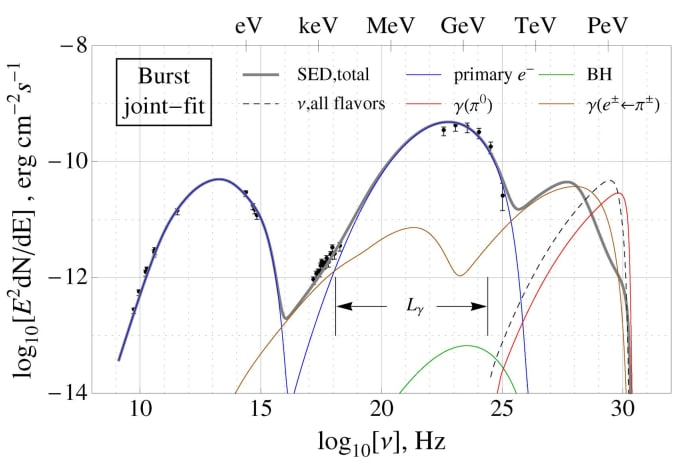
\includegraphics[width=10cm]{Plots/01_5_astroparticle/sed.jpeg}
    \caption{Different components of the blazar SED. The black dashed line on the right shows the neutrino emission spectrum around $\si{\peta\electronvolt}$ energies \cite{sed}.}
    \label{fig:sed}
\end{figure}
Accordingly, without more complex models, blazars cannot be significantly responsible for neutrinos with energies below $\si{\peta\electronvolt}$ \cite{blazar}.
Approaches for neutrinos of lower energies include the approach of the hadronuclear channel by assuming a high particle density in the emission volume of the blazar \cite{eichmann}.
Better sources for neutrinos in the $\si{\tera\electronvolt}$ range are starburst galaxies.

\subsection{Starburst Galaxies}
%- starburstgalaxies are galaxies with star formation at extreme levels\\
%- example: Arp 220\\
%- consists of two nuclei\\
%- star formation rate of > 100 sun mass per year\\
%- "Arp 220 is a hadronic cosmic ray calorimeter where all the power in %cosmic rays is absorbed within the nuclear starburst zones"\\
%- up to a hundred percent proton calorimeters\\
%- pp interaction -> pions -> 1.neutrino + charged lepton\\
%- flux of 1. neutrino is about $\num{6e-%12}\si{\giga\electronvolt\centi\meter\tothe{-2}\second\tothe{-1}}$ at %$\SI{0.1}{\peta\electronvolt}$\\
%\cite{starburst}
%- neutrinos from pp have a typical energy of about %$\SI{2}{\peta\electronvolt}$
%\cite{starburst2}

Apart from blazars, starburst galaxies are candidates for the production of neutrinos of energies up to about $\SI{2}{\peta\electronvolt}$ \cite{starburst2}.
These are galaxies in which stars form at extreme levels.
One example is Arp 220, an object consisting of two nuclei surrounded by dense molecular gas.
The gas turns the object almost completely into a cosmic ray calorimeter.
Under certain model assumptions, the $pp$-interactions provide a neutrino flux for the first part of the interaction of about $\num{6e-12}\si{\giga\electronvolt\centi\meter\tothe{-2}\second\tothe{-1}}$ at $\SI{0.1}{\peta\electronvolt}$ \cite{starburst}.
The neutrino emission spectrum can be seen in figure \ref{fig:starburst} showing an emission of neutrinos in a wide energy range.
\begin{figure}
    \centering
    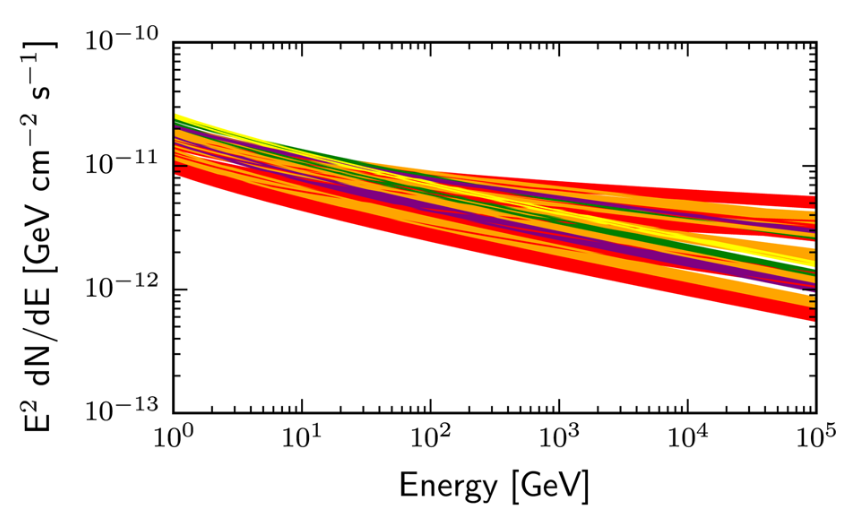
\includegraphics[width=10cm]{Plots/01_5_astroparticle/starburst_flux.png}
    \caption{Neutrino emission spectrum bands, as a function of energy in starburst galaxies. The different colours represent different combinations of fractions of the two nuclei of Arp 220 and are not important here.\todo{style} Important is the steady emission of low-energy to high-energy neutrinos \cite{starburst}.}
    \label{fig:starburst}
\end{figure}
